
\documentclass{standalone}
\usepackage{tikz}
\usetikzlibrary{hobby}
\usetikzlibrary{calc}
\usetikzlibrary{math}


\begin{document}
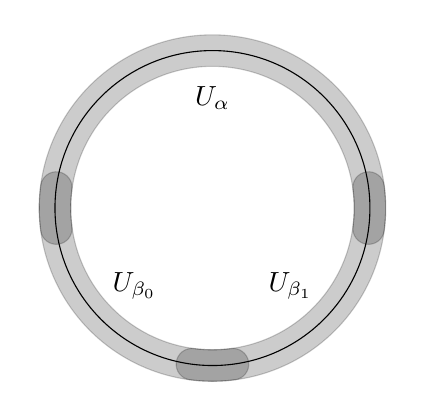
\begin{tikzpicture}
\tikzmath{\overlap=7.5;}

\draw (0,0) circle(2);


\foreach \s/\e in {-\overlap/180 + \overlap, 180 - \overlap/270 + \overlap, 270 - \overlap/360 + \overlap}
	\draw[fill, opacity=0.2] ([shift=(\s:1.8)]0,0) arc (\s:\e:1.8) arc (180 + \e:\e:0.2) arc (\e:\s:2.2) arc (360 + \s:180 + \s:0.2);
	% \draw[fill, opacity=0.2] ([shift=(\start-\overlap:1.8)]0,0) arc (\start-\overlap:\end + \overlap:1.8) arc (360 + \start + \overlap:\end + \overlap:0.2) arc (\end + \overlap:\start-\overlap:2.2) arc (360 + \start - \overlap:180 - \start + \overlap:0.2);
	% \draw[fill, opacity=0.2] ([shift=(360 + \overlap:1.8)]0,0) arc (360 + \overlap:270 - \overlap:1.8) arc (-\overlap:180 - \overlap:0.2) arc (180 - \overlap:360 + \overlap:2.2) arc(\overlap:180 + \overlap:0.2);

\draw (90: 1.4) node {$U_\alpha$};
\draw (225:1.4) node {$U_{\beta_0}$};
\draw (315:1.4) node {$U_{\beta_1}$};
\end{tikzpicture}
\end{document}
